\documentclass[12pt, UTF8, AutoFakeBold]{ctexart}  % , openany
\usepackage{xeCJK}
\usepackage{amsfonts}  % \mathbb 黑版粗体支持
\usepackage{amsmath}
% \numberwithin{equation}{section} % 公式与章节关联
\renewcommand\theequation{\arabic{section}-\arabic{equation}} % 公式引用输出样式
\usepackage{listings}  % 代码块
\usepackage{newtxtt, newtxmath}
\usepackage{times}
\usepackage{pdfpages}
\usepackage{geometry}  % 页面尺寸
\usepackage{enumerate}
\usepackage{graphicx}
\usepackage{float}
\usepackage{subfigure} % 插入多图片
\usepackage{caption}
\usepackage{fancyhdr} % 页眉页脚
%------- 页眉页脚样式 -------%
\pagestyle{fancy}
\fancyhf{}
\fancyhead[C]{\song\xiaowu{东北林业大学本科毕业论文}}
% \fancyhead[CO]{\thechapter}
\fancyfoot[C]{\xiaowu{-\thepage-}}
\renewcommand{\headrulewidth}{0.4pt}
%------- 双线页眉的设置 -------%
\makeatletter %双线页眉
\def\headrule{{\if@fancyplain\let\headrulewidth\plainheadrulewidth\fi%
\hrule\@height 1.0pt \@width\columnwidth\vskip1pt%上面线为1pt粗
\hrule\@height 0.5pt\@width\columnwidth  %下面0.5pt粗
\vskip-2\headrulewidth\vskip-1pt}      %两条线的距离1pt
  \vspace{6mm}}     %双线与下面正文之间的垂直间距
\makeatother

% 更改插图标题格式
\renewcommand {\thetable} {\thesection{}-\arabic{table}} 
\renewcommand {\thefigure} {\thesection{}-\arabic{figure}}
\captionsetup{labelformat=default,labelsep=space} %去除冒号

\geometry{a4paper, left=2.4cm, top=2.4cm, right=2.4cm, bottom=2.4cm}  % 页边距

\setCJKmainfont{SimSun}
\setmainfont{Times New Roman}

% 代码块设置
\lstset{
  basicstyle=\xiaowu\fontspec{Consolas}, 
  columns=fixed,       
  % numbers=left,                                        % 在左侧显示行号
  % numberstyle=\tiny\color{gray},                       % 设定行号格式
  frame=none,                                          % 不显示背景边框
  backgroundcolor=\color[RGB]{245,245,244},            % 设定背景颜色
  keywordstyle={                                       % 设定关键字颜色
    \color[RGB]{40,40,255}
    \fontspec{Consolas}
  },               
  numberstyle=\footnotesize\color{darkgray},           
  commentstyle=\it\color[RGB]{0,96,96},                % 设置代码注释的格式
  stringstyle=\rmfamily\slshape\color[RGB]{128,0,0},   % 设置字符串格式
  showstringspaces=false,                              % 不显示字符串中的空格
  language=python,                                     % 设置语言
}


\title{基于深度学习的小麦病害分类模型特征分析}
\date{}
\author{马群}
% \date{2019年2月22日}

% 英文摘要
\newcommand{\enabstractname}{Abstract}
\newenvironment{enabstract}{%
    \par\small
    \noindent\mbox{}\hfill{\bfseries \enabstractname}\hfill\mbox{}\par
    \vskip 2.5ex}{\par\vskip 2.5ex}

\begin{document}

% 定义字体
\newcommand{\song}{\CJKfamily{song}}    % 宋体
\newcommand{\fs}{\CJKfamily{fs}}        % 仿宋体
\newcommand{\kai}{\CJKfamily{kai}}      % 楷体
\newcommand{\hei}{\CJKfamily{hei}}      % 黑体
\newcommand{\li}{\CJKfamily{li}}        % 隶书

\newcommand{\yihao}{\fontsize{26pt}{36pt}\selectfont}         % 一号, 1.4 倍行距
\newcommand{\erhao}{\fontsize{22pt}{28pt}\selectfont}         % 二号, 1.25倍行距
\newcommand{\xiaoer}{\fontsize{18pt}{18pt}\selectfont}        % 小二, 单倍行距
\newcommand{\sanhao}{\fontsize{16pt}{24pt}\selectfont}        % 三号, 1.5倍行距
\newcommand{\xiaosan}{\fontsize{15pt}{22pt}\selectfont}       % 小三, 1.5倍行距
\newcommand{\sihao}{\fontsize{14pt}{21pt}\selectfont}         % 四号, 1.5 倍行距
\newcommand{\banxiaosi}{\fontsize{13pt}{19.5pt}\selectfont}   % 半小四, 1.5倍行距
\newcommand{\xiaosi}{\fontsize{12pt}{18pt}\selectfont}        % 小四, 1.5倍行距
\newcommand{\dawu}{\fontsize{11pt}{11pt}\selectfont}       % 大五号, 单倍行距
\newcommand{\wuhao}{\fontsize{10.5pt}{15.75pt}\selectfont}    % 五号, 单倍行距
\newcommand{\xiaowu}{\fontsize{9pt}{9pt}\selectfont}    % 小五, 单倍行距
\newcommand{\zerospace}{\hspace{0pt}}
\newcommand{\onespace}{\hspace{1pt}}

% \begin{center}
    \includegraphics[height=1.53cm,width=7.00cm,bb=0 0 887 191]{resource/nefu_pic.png}
\end{center}
  \includepdf{cover/cover.pdf}

  \maketitle
  \begin{abstract}
    为了实时监控小麦病害情况并及时采取防治措施,找出一种适合分类处理小麦常见病害的神经网络模型。
    本文首先以小麦病害图片资料为基础,经过挑选、裁剪后对图像进行序列化操作形成数据集,
    然后通过构建的多个深度神经网络模型进行学习,并利用随机梯度下降法进行学习过程控制。
    然后在此基础上改进表现较差的神经网络模型,在两个维度上形成对比,以此寻找最适合处理
    小麦病害分类问题的深度神经网络模型。实验结果表明,在参与实验的多个神经网络结构中,
    以卷积神经网络(convolutional neural networks,CNN)表现最为出众,
    整体识别准确率达99\%,(交叉)验证准确率在(validation accuracy)75\%左右。
    这表明卷积神经网络在小麦常见病害的识别中是有效且可行的,为小麦病害实时分析提供了有效分析手段。

    \leftline{\textbf{关键字 } \@ 小麦病害;卷积神经网络;卷积深度置信网络}
\end{abstract}
\newpage

\begin{center}
    \fontsize{18pt}{18pt}\textbf{Feature analysis of wheat disease classification model based on deep learning}
\end{center}
\begin{enabstract}
    This is the abstract in English.    This is the abstract in English.    This is the abstract in English.    This is the abstract in English.    This is the abstract in English.

    \leftline{\textbf{Keywords } \@ Wheat disease; Convolutional Neural Network; Convolutional deep belief networks}
\end{enabstract}
\newpage

  \tableofcontents % 目录
  \newpage

  \section{\hei\xiaoer\textbf{前言}}
  
\subsection{\textbf{研究背景及意义}}
小麦是我国三大粮食作物之一,其种植区域主要分布在长江以北的大部分地区,种植面积位居第二,仅次于水稻。
病害是影响小麦等农作物产量和质量的首要问题。全世界范围内小麦病害大约有200多种,每年造成的产量
损失约为15\%\textasciitilde20\%。在我国危害较严重的有三十多种,其中以白粉病(Wheat powdery mildew)、
锈病(Puccinia striiformis West,包括条锈、杆锈、叶锈)、叶枯病(Wheat leaf blotch)、
赤霉病等在我国主要小麦产地分布较广,为害较为严重\cite{CGRIS}。

传统形式的小麦病虫害是依靠经验识别、人工喷施农药进行防治的。在大面积的小麦种植模式下,人工防
治不仅需要大量的人力物力,而且在喷施农药的过程中极为不安全。更进一步地讲,即使是在技术人员的
帮助下进行病害防治,也不能做到实时监控小麦病害情况、及时实施防治工作。因此如何做到实时监控并
报告小麦病害情况成为了现代农业生产中的重要目标。

自1980年机器学习被称为一个独立的方向开始,经过一代又一代人的努力,诞生出了大量经典的分类算法。
其中以朴素贝叶斯(Naive Bayes, NB)、Logistic回归(Logistic Regression, LR)、决策树
(Decision Tree, DT)、支持向量机(Support Vector Machine, SVM)等浅层机器学习模型最常用,
它们的出现为小麦病害的自动识别提供了有力的理论支持。但是这些经典分类算法的图像特征提取策略是基
于先验知识制定的,效率不高且不适合应用在大规模特征提取方面\cite{article1}。 近年来,由AlphaGo
带来的人工智能热潮使得深度学习一词出现在公共视野里。 深度学习是机器学习领域中一种以人工神经网络
为架构,通过数据进行表征学习的算法。

如此一来,将现代的深度学习技术与传统图像处理相结合的方式成为了农作物病害识别的新手段。深度学习在
图像处理领域的优势不仅仅在于能够准确地提取特征,还在于它通过处理大量图像数据时能不断地自我学习并
取得更高的准确率。

在以深度学习为主要手段的图像处理过程中,卷积神经网络模型对图像的处理由很高的优势,故本文研究的内
容会以卷积神经网络为基础,通过建立不同结构的神经网络模型并加以比较,找出最适合小麦病害识别的深度
网络模型。
 
  \subsection{\hei\xiaosan\textbf{农作物病害识别的国内外研究现状}}
  \subsubsection{\hei\sihao\textbf{国内研究现状}}
    国内将深度学习应用在图像处理尤其是农作物病害识别方面的研究起步较晚,大多数
    在机器学习背景下开始此领域研究的,近年来该领域的研究呈现井喷式发展,并
    取得了许多卓有成效的识别技术。
    2009年,王守志等(王守志等,2009)实现了基于核K-均值聚类方法的玉米叶部病害识别,
    实验涉及的4种玉米病害识别准确率达82.5\% \cite{王守志2009基于核};
    2011年,陈丽等(陈丽等,2011)提出了一种基于图像处理技术和概率神经网络技术的玉米
    叶部病害识别方法,利用遗传算法优化选择出4个分类能力强的分类特征,由概率网络(PNN)
    分类器识别病害,平均识别准确率为90.4\%,高于BP神经网络\cite{陈丽2011概率神经网络在玉米叶部病害识别中的应用};
    2012年,张建华等(张建华等,2012)提出了一种在自然条件下基于粗糙集和BP神经网络的
    棉花病害识别方法,准确识别了4种棉花病害,平均识别准确率达到92.72\% \cite{张建华2012基于粗糙集和};
    王树文等(王树文等,2012)利用基本图像处理方法对黄瓜叶部病害图像进行处理,综合运用
    二次分割、形态学滤波得到病斑区域。提取三种特征并采用BP算法训练多层前向人工神经网络
    对黄瓜病害进行分类,检测系统的黄瓜叶部病害平均识别精度为95.31\% \cite{王树文2012基于图像处理技术的黄瓜叶片病害识别诊断系统研究};
    2013年,张飞云等(张飞云等,2013)利用量子神经网络进行玉米病害分类识别,对玉米灰斑病、
    玉米普通锈病和玉米小斑病的识别准确率达92.5\%、97.5\%和92.5\%,高于误差反向传播神经网
    络法的识别率(分别为90.0\%、90.0\%和92.5\%),可用于玉米叶部病害识别\cite{张飞云2013基于量子神经网络和组合特征参数的玉米叶部病害识别};
    2014年,余秀丽等(余秀丽等,2014)设计并实现了一种基于SVM(Support Vector Machine,
    支持向量机)的小麦叶部常见病害识别方法。随机试验结果表明,利用所提取的特征可以有效地
    实现小麦叶部常见病害的识别,基于形状特征综合识别率可达99.33\%,利用支持向量机算法进
    行小麦病害叶片识别是有效的、可行的\cite{余秀丽2014基于};
    2015年,谭文学等(谭文学等,2015)设计了深度学习神经网络的果蔬果体图像识别方法,基于
    对网络误差的传播分析,提出弹性动量的参数学习方法,以苹果为例进行果体病理图像的识别试验。
    结果表明,该方法召回率为98.4\% \cite{谭文学2015基于弹性动量深度学习神经网络的果体病理图像识别};
    2018年,张航等(张航等,2018)提出了一种基于卷积神经网络的小麦病害识别方法,构建一个
    具有五层结构的深度学习模型并利用随机梯度下降法进行学习过程控制,其综合识别率可达99\% \cite{张航2018一种基于卷积神经网络的小麦病害识别方法}。

  \subsubsection{\hei\sihao\textbf{国外研究现状}}
    国外关于农作物病害识别的研究起步较早,在上世纪九十年代已有多种识别方法被提出。
    在早期的处理方法大多是对病害图像进行前期处理,包括图像分割、滤波、简单分类等技术,
    或是辅助以人工分析,然后再结合农作物病理学知识对处理后的数据进行分类识别。
    1997年,Tucker与Chakraborty(Tucker et al.,1997)提供了一种专用软件,可以检测
    向日葵和燕麦叶片上的病变,提供病变数量和类型以及病害严重程度的数据,但是该软件的分类
    准确率达不到预想程度 \cite{tucker1997quantitative};
    1999年,Sasaki等(Sasaki et al.,1999)使用光谱反射特性和滤光片图像构建了一个植物
    病害自动诊断系统,发现500,600和650mm的滤光镜图像比其他滤光镜图像更适合于识别,在
    创建鉴别参数对健康叶片和患病叶片进行分类后,达到了5\%或更小的误差率\cite{sasaki1999automatic}。

    由于图像处理技术的限制,早期的农作物病害识别技术并不能满足人们的要求。近年来,随着
    图像处理和人工智能的发展,机器学习应用到农作物病害识别领域的例子越来越多。
    2008年,Phadikar和Sil等(Phadikar et al.,2008)介绍了一种基于水稻植株感染图像的
    水稻病害检测系统,该系统使用图像生长、分割技术处理感染部分,然后使用SOM神经网络将四种
    叶子的感染部分进行分类处理,实验结果令人满意\cite{phadikar2008rice};
    2014年,Mathura与Uttar Pradesh(Mathura et al.,2014)介绍了一种基于邻近像素点像素
    强度的改进和差直方图,与梯度滤波器相配合使用可以对苹果病害的检测达到99\%的准确率 \cite{dubey2014fruit};
    2016年,Sladojevic等(Sladojevic et al.,2016)实现了最新一代的卷积神经网络(CNN),
    该模型能够识别健康叶片中的13种不同类型的植物病害,实验结果的平均精确度达到了96.3\% \cite{sladojevic2016deep};
    2017年,Fuentes和Yoon等(Fuentes et al.,2017)提出了一种深度学习方法来检测番茄病害,
    该方法含有三种神经元架构:基于区域的快速卷积网络(Faster R-CNN)、基于区域的全卷积网络
    (R-FCN)和单发多核检测器(SSD),实验结果表明,该系统能有效识别九种不同类型的病虫害\cite{fuentes2017robust};

  \subsection{\hei\xiaosan\textbf{深度学习与神经网络的发展}}
  深度学习是机器学习领域中一种以人工神经网络为架构,根据数据进行表征学习的算法。同时它也是
  神经网络、最优化方法、模式识别、人工智能等领域的交叉学科,主要解决了贡献度的分配问题。

  对于深度学习的研究最早可以追溯到1943年,由神经科学家麦卡洛克(W.S.McCulloch)和数学家皮
  兹(W.Pitts)建立了神经网络和数学模型,称为MCP模型。该模型是按照生物神经元的结构和工作
  原理构造出来的一个抽象的简化模型,所谓的“模拟大脑”由此诞生,深度学习和人工神经网络的大门
  由此开启\cite{mcculloch1990logical}。1958年,计算机科学家罗森布拉特(Rosenblatt)提出
  了两层神经元组成的神经网络,称之为“感知器”(Perceptrons)。第一次将MCP模型用于机器学习分
  类。“感知器”算法使用MCP模型对输入的多维数据进行二分类,且能够使用梯度下降法从训练样本中自
  动学习更新权值。1962年,该方法被证明能够收敛,理论与实践效果引起第一次神经网络浪潮。

  神经网络之父Geoffery Hinton在1986年发明了适用于多层感知器(MLP)的BP(Backpropagation)
  算法,并采用Sigmoid进行非线性映射,有效解决了非线性分类和学习的问题。引起了神经网络
  的第二次热潮。Sigmoid 函数是一个在生物学中常见的S型的函数,也称为S型生长曲线。在信息科学
  中,由于其单增以及反函数单增等性质,Sigmoid函数常被用作神经网络的阈值函数,将变量映射到0,
  1之间。90年代中期,支持向量机(Support Vector Machine,SVM)算法诞生等各种浅层机器学习
  模型被提出,SVM也是一种有监督的学习模型,应用于模式识别,分类以及回归分析等。支持向量机以
  统计学为基础,和神经网络有明显的差异,支持向量机等算法的提出再次阻碍了深度学习的发展。2006
  年Geoffrey Hinton和他的学生Ruslan Salakhutdinov提出了深层网络训练中梯度消失问题的解决方
  案:无监督预训练对权值进行初始化+有监督训练微调\cite{hinton2006reducing}。2011年,ReLU
  激活函数被提出,该激活函数能够有效的抑制梯度消失问题。

  2011年以来,微软首次将深度学习应用在语音识别上,取得了重大突破。微软研究院和Google的语音识别
  研究人员先后采用DNN技术降低语音识别错误率20%~30%,是语音识别领域十多年来最大的突破性进展。
  2012年,Hinton课题组为了证明深度学习的潜力,首次参加ImageNet图像识别比赛,其构建的CNN网络
  AlexNet在ImageNet评测上将错误率从26\%降低到15\%,在第二名(SVM方法)面前以压倒性的优势夺得
  冠军。也正是由于该比赛,CNN吸引到了众多研究者的注意。AlexNet的创新点在于:
  
  \begin{enumerate}[(1)]
    \dawu\item 首次采用ReLU激活函数,极大增大收敛速度且从根本上解决了梯度消失问题。
    \dawu\item 由于ReLU方法可以很好抑制梯度消失问题,AlexNet抛弃了“预训练+微调”的方法,完全采用
      有监督训练。也正因为如此,DL的主流学习方法也因此变为了纯粹的有监督学习。
    \dawu\item 扩展了LeNet5结构,添加Dropout层减小过拟合,LRN层增强泛化能力/减小过拟合。
    \dawu\item 第一次使用GPU加速模型计算。
  \end{enumerate}

  2016年3月,由谷歌(Google)旗下DeepMind公司开发的AlphaGo(基于深度学习)与围棋世界冠军、职业
  九段棋手李世石进行围棋人机大战,以4比1的总比分获胜;2016年末2017年初,该程序在中国棋类网站上
  以“大师”(Master)为注册帐号与中日韩数十位围棋高手进行快棋对决,连续60局无一败绩;2017年5月,
  在中国乌镇围棋峰会上,它与排名世界第一的世界围棋冠军柯洁对战,以3比0的总比分获胜。围棋界公认
  阿尔法围棋的棋力已经超过人类职业围棋顶尖水平。

  深度学习虽然已经成为众多科研领域的热门研究内容,但是目前还处于发展阶段,不管是理论方面还是实践
  方面都还有许多问题待解决,不过由于我们处在了一个“大数据”时代,以及计算资源的大大提升,新模型、
  新理论的验证周期会大大缩短,人工智能的开启必然会很大程度地改变这个世界。

  \subsection{\hei\xiaosan\textbf{论文结构和研究内容}}
  \subsubsection{\hei\sihao\textbf{主要研究内容}}
    本文以提高卷积网络在小麦病害图像识别的准确率为目标,提出了具有12层结构的卷积网络。
    针对前期实验的不足之处对网络结构加以更改,在得到了训练过程中表现良好的网络模型的模型之后,
    将其与经典卷积网络模型LeNet-5、AlexNet的实验结果进行比较,分析本文模型的长处与不足,验证
    该模型在小麦病害图像识别中的有效性。
    

  \subsubsection{\hei\sihao\textbf{论文结构}}
    第一章是引言,首先介绍了小麦病害图像识别的研究背景和意义,
    然后综述了深度学习与\zs 神经网络的\zs 发展历史及\zs 研究现状,
    最后介绍\zs 了本文的主要研究内容和章节安排。

    第二章主要介绍了卷积的基础理论知识,然后简单介绍了卷积神经网络的发展及其特点和主要结构层次。

    第三章搭建了一个结构上较新颖的卷积神经网络模型,并针对小麦病害识别加以修改,
    使其尽量符合预期要求。接下来主要介绍了实验内容,首先是数据源的获取和处理,然后是不同模型
    在相同数据源下的训练过程。

    第四章是针对该实验结果的分析以及对不同模型的结果加以对比,说明本文新模型的优势。
    然后对数据集的质量进行了解释,以及数据集对训练结果的影响。最后是对本文的总结分析。
  \newpage

  \section{\hei\xiaoer\textbf{卷积网络}}
    \subsection{卷积}
  卷积(Convolution)是分析数学中的一种积分变换的方法,是其中一个函数反转并平移后与另一个
  函数乘积的积分。设$f$与$g$是$\mathbf{R_1}$上的两个可积函数,做积分后的新函数就成为函数
  $f$与$g$的卷积:
  \[f*g=\int_{\tau \in A}f(\tau)g(t-\tau) d\tau\]

  卷积也经常应用在图像处理中,因为图像是一个二维结构,所以适合用二维卷积对图像做特征提取等操作。
  给定一个图像$\mathbf{I}\in \mathbb{R}^{M\times N}$,
  和滤波器 $\mathbf{K}\in \mathbb{R}^{M\times N}$,
  一般$m<<M$,$n<<N$,其卷积为:
  % \[y_{ij}=\sum_{u=1}^m \sum_{v=1}^n w_{uv}\cdot x_{i-u+1,j-v+1}\]
  \begin{equation}
    S(i,j)=(I*K)(i,j)=\sum_m \sum_n I(m,n)K(i-m,j-n)
    \label{Formula.Second.1}
  \end{equation}
  下式为二维卷积示例:
  \begin{equation}
    {\begin{pmatrix}
    2& 0& 1& 1& 1 \\
    -1& 0& -3& 0& 1\\
    2& 1& 1& -1& 0 \\
    0& -1& 1& 2& 1 \\
    1& 2& 1& 1& 1
    \end{pmatrix}} 
    \otimes 
    {\begin{pmatrix}
      1& 0& 0\\
      0& 0& 0\\
      0& 0& -1
    \end{pmatrix}}
    =
    {\begin{pmatrix}
      -1& 1& -1\\
      2& 2& 4\\
      -1& 0& 0\\
    \end{pmatrix}}
    \label{Formula.Second.2}
  \end{equation}

  卷积是可交换的,我们可以等价地把(2-1)式写作:
  \begin{equation}
    (\ref{Formula.Second.1}) \Leftrightarrow S(i,j)=(K*I)(i,j)=\sum_m \sum_n I(i-m,j-n)K(m,n)
    \label{Formula.Second.3}
  \end{equation}
  (\ref{Formula.Second.3})式也被称为I和K的互相关(Cross-Correlation),它是一个衡量两个序列相关性的函数。通过(\ref{Formula.Second.1})、
  (\ref{Formula.Second.3})两式对比可知,卷积和互相关的区别仅仅在于卷积核是否进行了翻转(Flip)。许多机器学习库中实现的
  “卷积运算”其实是互相关函数,之所以称之为卷积运算,这是因为卷积核的特征提取能力与其是否翻转无关。在训练
  过程中,学习算法会在核合适的位置自动更新为恰当的值,所以一个基于互相关学习算法所学习到的核,是使用卷
  积运算所学到的核的翻转。

  数字图像是二维图像用有限数字数字像素的表示\upcite{wiki:数字图像},对数字图像做卷积操作其实是在图像上滑动一个卷积核(即滤波器),
  将图像点上的像素值与卷积核对应位置的值相乘,然后将相乘后所有的值相加,作为特征图像上对应位置的像素值。
  图\ref{Figure.Second.1}展示了式(\ref{Formula.Second.2})中反转前后的卷积核在小麦锈病图像中特征提取效果的对比图。
  \begin{figure}[H]
    \centering %图片全局居中
    \subfigure[原图]{
      \includegraphics[width=.2\textwidth]{resource/second/rust.jpg}
    }
    \subfigure[互相关]{
      \includegraphics[width=.2\textwidth]{resource/second/nconv.jpg}
    }
    \subfigure[卷积]{
      \includegraphics[width=.2\textwidth]{resource/second/conv.jpg}
    }
    \caption{卷积核的翻转对特征提取的影响}
    \label{Figure.Second.1}
  \end{figure}
  

  
  \subsection{\hei\xiaosan\textbf{卷积网络简介}}
    卷积网络(Convolutional Network),也叫卷积神经网络(Convolutional Neural Network,CNN),
    是一种具有局部连接、权重共享等特性的深层前馈神经网络,专门用来处理具有类似网格结构的数据的神经网络。
    

    1962年,Hubel和Wiesel通过对猫脑视觉皮层的研究,首次提出了一种新的概念——“感受野”
    (Receptive Field),对后来人工智能网络的发展起了很大的推动作用\upcite{hubel1962receptive}。
    感受野是受生物学上感受野的机制而提出,在生物学上描述的是神经系统的一些神经元的特性。
    而在人工神经网络中,感受野指的是指的是卷积神经网络层输出的特征向量上的像素点对应的
    输入图像上的区域,通俗地讲,就是特征向量上的一个点对应的输入图像上的区域。1980年,Fukushima
    \upcite{fukushima1982neocognitron}基于生物神经学的感受野理论提出了神经认知机和权重
    共享的卷积神经层,这被视为卷积神经网络的雏形。1989年,LeCun
    将反向传播算法与权值共享的卷积神经层相结合,发明了卷积神经网络,并首次将卷积神经网络成功
    地应用到美国邮局的手写字符识别程序中\upcite{lecun1989backpropagation}。1998年,LeCun提出了
    经典卷积神经网络模型LeNet-5,该模型是第一个成功应用于图像数字识别的卷积神经网络\upcite{lecun1998gradient}。
    
 
  \subsection{\hei\xiaosan\textbf{卷积网络的特点}}
    % 卷积神经网络由神经认知机模型(Neocognitron)演变而来,由于其具有局部
    % 区域连接、权值共享、池化的结构特点,使得卷积神经网络在图像处理领域表现出色。与
    % 其他神经网络相比,卷积神经网络的特殊性表现在权值共享与局部连接等方面。权值共享使
    % 得卷积神经网络的网络结构与生物神经网络更加类似,从而更容易从中提取特征。局部连接
    % 不像传统神经网络那样,两个相连的网络层之间只有部分神经元互相连接,这两个特点很大
    % 程度上降低了网络模型的复杂度,减少了参数的数目,也提高了整个神经网络的训练效率。
    卷积运算通过三个重要的思想帮助改进深度学习系统:稀疏交互(Sparse Interactions)、
    参数共享(Parameter Shareing)和等变表示(Equivariant Representations)。
    
    稀疏交互的本质是对全连接的规避,这是通过使核的大小远小于输入的大小来达到的。当处理一
    张图像时,输入的图像可能包含几十万个像素点,但是我们可以使用只有数十个像素点的卷积核来
    达到提取特征的目的。这意味着我们不仅可以存储更少的参数,而且还大大减少了计算量,提高了
    统计效率。稀疏交互的图形化表示如图\ref{Figure.Second.2}所示。
    \begin{figure}[htbp]
      \centering
      \includegraphics[width=.4\textwidth, natwidth=624, natheight=577]{resource/second/sparse.png}
      \caption{稀疏交互}
      \label{Figure.Second.2}
    \end{figure}
    
    参数共享是指在一个模型的多个函数中使用相同的参数。在传统的神经网络中,当计算一层的
    输出时,权重矩阵的每一个元素只使用一次,当它乘以输入的一个元素之后就再也用不到了。
    在卷积神经网络中,核的每一个元素都作用在输入的每一个位置上。参数共享保证了我们只需
    要学习一个参数集合,而不是每一个位置都需要学习一个新的集合。因此,卷积在存储需求和
    统计效率方面极大地优于稠密矩阵的乘法运算。

    在处理图像数据时,卷积产生了一个二维映射来表明某些特征在输入中出现的位置。
    如果我们移动输入中的图像,它的表示也会在输出中移动同样的量,这种性质就叫做等变表示。
    对于卷积来说,参数共享的特殊形式使得神经网络层具有对平移等变的性质。如果一个函数满足
    输入改变,输出也以同样的方式改变这一性质,我们就说它是等变的。特别的,如果函数$f(x)$与
    $g(x)$满足$f(g(x))=g(f(x))$,我们就说$f(x)$对于变换$g$具有等变性。对于卷积来说,
    如果令$g$是输入的任意平移函数,那么卷积函数对于$g$具有等变性。

  
  \subsection{\hei\xiaosan\textbf{卷积网络的结构}}
    卷积网络一般由数个卷积层(Convolutional layer)、池化层(Pooling 
    layer)、全连接层及输出层交叉堆叠而成,卷积层和池化层一般会取多个,采用卷积层和
    池化层交替堆叠的模式。卷积层可以并行地计算多个卷积产生一组线性输出,每一个线性激活响应
    将会通过一个非线性的激活函数,例如线性整流激活函数。然后使用池化层来进一步调整这一层的输出。
    最后添加0~2个全连接层以输出最终结果。
    目前,整个网络结构趋向于使用更小的卷积核(比如11和33)以及更深的网络结构。
    此外,由于卷积的操作性越来越灵活,池化层的作用也变得越来越小,因此目前比较流行的卷积网络中
    池化层的比例也越来越低,趋向于全卷积网络。
    
   

  \newpage

  \section{\hei\xiaoer\textbf{基于卷积网络的小麦病害图像识别}}
  %图表序号清零
\setcounter{table}{0}
\setcounter{figure}{0}

\subsection{\hei\xiaosan\textbf{本文卷积网络结构}}
  \begin{figure}[H]
    \centering
    \includegraphics[width=.5\textwidth]{resource/NewbNet.png}
    \caption{网络结构及输入输出}
    \label{Figure.Third.1}
  \end{figure}

  \begin{figure}[H]
    \centering
    \includegraphics[width=.5\textwidth]{resource/graph.png}
    \caption{网络结构及数据流}
    \label{Figure.Third.2}
  \end{figure}


  本文卷积网络模型中每一层的输入输出由图\ref{Figure.Third.1}所示,相对应网络层的操作由
  图\ref{Figure.Third.2}所示。

  第一层和第二层为卷积层,它们的过滤器大小均为$3\times3$,深度为32,不使用全零填充,步长为1。
  第一层接受的输入层大小为$100\times100\times3$,所以输出的尺寸为$100+3-1=98$,深度为32。
  这一层共有$3\times3\times1\times32+32=320$个参数,其中32个为偏置。下一层节点矩阵有
  $98\times98\times32=307328$个节点,每个节点和$3\times3=9$个当前层节点相连,所以本卷积层
  共有$307328\times(9+1)=3073280$个连接。同理,第二层中共有$96\times96\times32\times(3\times3+1)=2949120$个连接。

  第三层为最大池化层,是一个$96\times96\times32$的节点矩阵。在本层中使用的过滤器大小为$2\times2$,步长为2.
  所以本层的输出大小为$48\times48\times32$。

  第四层为Dropout层,该层是Hinton\upcite{hinton2012improving}为了防止过拟合、提高
  神经网络的性能而提出的。该层会随机丢弃一些神经元,dropout rate为0.25。

  第五至八层结构与前四层相似,不过为了提取更深的特征,将深度增加为64层。

  第九层Flatten操作将输入$22\times22\times64$的张量展平为1维$1\times30976$的张量,
  为下一层的全连接操作做准备。

  第十层的全连接层(Dense)使用ReLU(RecitifiedLinearUnit,ReLU)作为激活函数。
  ReLU即线性整流函数,指代数学中的斜坡函数:$f(x)=max(0,x)$\upcite{wiki:ReLU}。
  该层输入大小为$30976$,输出节点个数为256个,总共参数为$30976\times256+256=7930112$个。

  第十一层仍为Dropout层,随机丢弃率为0.5。

  第十二层为全连接层,该层使用Softmax函数作为激活函数,该函数能将一个含任意实数的K维向量$\mathbf{Z}$
  “压缩”到另一个K维实向量$\sigma(\mathbf{Z})$中,并使得每一个元素的值域均在$(0,1)$之间,并且所有原色的和为1\upcite{wiki:Softmax}。
  该函数的形式通常由下式给出:
  \[
    \sigma(\mathbf{Z})_j=\frac{e^{z_j}}{\sum^\mathbf{K}_{k=1} e^{z_k}} \quad for\ j=1, \dots,\mathbf{K}
  \]
  该层输入大小为$256\times1$的张量,输出大小为3,即小麦病害类别个数。




\subsection{\hei\xiaosan\textbf{LeNet-5和AlexNet结构简介}}
  \begin{figure}[htbp]
    \centering
    \includegraphics[width=\textwidth, natwidth=1612, natheight=482]{resource/second/LeNet-5.png}
    \caption{LeNet-5网络结构}
    \label{Figure.Third.3}
  \end{figure}
  LeNet-5模型接受的输入层大小为$32\times32\times1$。
  第一个卷积层过滤器尺寸为$5\times5$,深度与输出深度通为6,步长为1,
  输出尺寸为$32-5+1=28$。该层共有$5\times5\times1\times6+6=156$个参数,其中6个为偏置。
  下一层的节点矩阵有$28\times28\times6=4704$个节点,每个节点和$5\times5=25$给节点相连,所以本层共有
  $4704\times(25+1)=122304$个连接。

  % 第二层池化层的输入是$28\times28\times6$的节点矩阵,过滤器大小为$2\times2$,步长为2。
  % 第三层是输入大小为$14\times14\times6$的卷积层,卷积核大小为
  % $2\times2$,步长为2。第四层是输入大小为$10\times10\times6$的卷积层,过滤器大小为$2\times2$,步长为2。
  第二至四层均为卷积核大小$2\times2$、步长为2的卷积层。第五至七层均为全连接层,最后一层的输出为10个预测值。


  \begin{figure}[htbp]
    \centering
    \includegraphics[width=\textwidth]{resource/second/AlexNet.png}
    \caption{AlexNet网络结构}
    \label{Figure.Third.4}
  \end{figure}
  AlexNet的输入图片大小为$224\times224\times3$,第一个卷积层使用96个较大的卷积核($11\times11$)
  步长为4;接着是LRN层;在之后是一个过滤器为$3\times3$的最大池化层,步长为2。接下来的卷积层中使用
  的卷积核都是$3\times3$或$5\times5$的大小,并且步长均为1。最大池化层依然是$3\times3$,步长为2。
  最后是三层均为全连接层,输出1000个预测结果。

\subsection{\hei\xiaosan\textbf{实验步骤及操作}}
  \subsubsection{\hei\sihao\textbf{数据的获取及处理}}
    

    实验所用的图片均来自网络。首先利用Python爬虫分别在百度图片和谷歌图片上爬取小麦的白粉病、
    叶枯病、锈病图片,保存至本地文件夹并做好备份。手工去除不清晰、含水印等劣质图片后,使用Python
    脚本将原始图片切割为多份$300px\times300px$的图片。然后将这些图片按3:1:1的比例随机分为train、
    test、evaluate三个数据集,使用Python将全部图片的尺寸缩小为$100px\times100px$后转为numpy数组,
    最后将这些数组序列化为$*.npy$文件,这样的做法
    为重复实验省去了磁盘$IO$和图片处理操作的时间。数据集的样本和比例分布如图\ref{Figure.Third.5}所示:

    \begin{figure}[htbp]
      \centering
      \includegraphics[width=.65\textwidth]{resource/second/data_ratio.bmp}
      \caption{实验数据分布}
      \label{Figure.Third.5}
    \end{figure}

    \begin{figure}[H]
      \centering %图片全局居中
      \subfigure[叶枯病]{
        \begin{minipage}[t]{.2\textwidth}
          \includegraphics[width=\textwidth]{resource/third/blight(1).jpg} \
          \includegraphics[width=\textwidth]{resource/third/blight(2).jpg} \
          \includegraphics[width=\textwidth]{resource/third/blight(3).jpg} 
        \end{minipage}
      }
      \subfigure[白粉病]{
        \begin{minipage}[t]{.2\textwidth}
          \includegraphics[width=\textwidth]{resource/third/powdery(1).jpg} \
          \includegraphics[width=\textwidth]{resource/third/powdery(2).jpg} \
          \includegraphics[width=\textwidth]{resource/third/powdery(3).jpg} 
        \end{minipage}
      }
      \subfigure[锈病]{
        \begin{minipage}[t]{.2\textwidth}
          \includegraphics[width=\textwidth]{resource/third/rust(1).jpg} \
          \includegraphics[width=\textwidth]{resource/third/rust(2).jpg} \
          \includegraphics[width=\textwidth]{resource/third/rust(3).jpg} 
        \end{minipage}
      }
      \caption{数据样本}
      \label{Figure.Third.6}
    \end{figure}


  \subsubsection{\hei\sihao\textbf{卷积网络模型的建立}}
    在机器学习异常火热的今天,越来越多的机器学习库可供大家学习。本文使用最受欢迎的深度学习框架
    $TensorFlow$搭建卷积网络模型,具体环境为:

    {\hei\dawu
    \begin{itemize}
      \item 操作系统:Windows 10 x64 Version 1809
      \item 处理器:Intel(R) Core(TM) i7-6700HQ CPU @ 2.60GHz
      \item 显卡:Geforce GTX 950M
      \item 软件环境:
            \begin{itemize}
              \item Python 3.6.8 64-bit
              \item tensorflow-gpu 1.12.0
              \item keras 2.1.6-tf
              \item tensorboard 1.12.1
            \end{itemize}
    \end{itemize}
    }

    在TensorFlow中已经集成了Keras,它是使用Python编写的高级神经网络API,
    能够以TensorFlow作为后端运行。实验中为快速搭建卷积网络,使用Keras可节省大量时间。
    以下即为核心代码:

    \begin{lstlisting}
  model = Sequential()
  model.add(Conv2D(32, (3, 3), activation='relu', input_shape=(100, 100, 3)))
  model.add(Conv2D(32, (3, 3), activation='relu'))
  model.add(MaxPooling2D(pool_size=(2, 2)))
  model.add(Dropout(0.25))
  model.add(Conv2D(64, (3, 3), activation='relu'))
  model.add(Conv2D(64, (3, 3), activation='relu'))
  model.add(MaxPooling2D(pool_size=(2, 2)))
  model.add(Dropout(0.25))
  model.add(Flatten())
  model.add(Dense(256, activation='relu'))
  model.add(Dropout(0.5))
  model.add(Dense(3, activation='softmax'))
  sgd = SGD(lr=0.0001, decay=1e-6, momentum=0.01, nesterov=True)
  model.compile(loss='categorical_crossentropy', optimizer=sgd, metrics=['accuracy'])
    \end{lstlisting}

    为了便于实验后的数据分析,需要在代码中加入回调函数$keras.callbacks.TensorBoard$,
    设置了必要的参数后,程序在执行时便会在指定的文件夹写入运行过程的日志文件以供分析。

  \newpage
  
  \section{\hei\xiaoer\textbf{实验结果分析}}
  %图表序号清零
\setcounter{table}{0}
\setcounter{figure}{0}

\subsection{\hei\xiaosan\textbf{参数优化}}

  不同于其他一些传统的黑盒机器学习方法,卷积网络所提取的
  图像特征在训练过程中是可视的,这不仅让人们对于卷积网络的工作过程
  有直观的了解,更能够帮助进行下一步的工作。在卷积网络的前向传播过程中
  部分卷积层滤波器提取的特征结果如图所示。

  \begin{figure}[H]
    \centering
    \includegraphics[width=.5\textwidth]{resource/数据分布.bmp}
    \caption{数据分布}
    \label{Figure.Fourth.1}
  \end{figure}

  为了改进本文模型的性能,在实验初期进行了不同迭代次数(分别为10000次、20000次)的实验,
  在图\ref{Figure.Fourth.2}中以[橙-深蓝]、[红-浅蓝]图像对应其测试集和验证集的准确率;而
  [粉-绿]图像代表了卷积网络初步优化后的效果。验证准确率在70\%\textasciitilde75\%徘徊的
  原因来自于数据集:因为数据来自百度和谷歌图库,而这些图片是从各个网页上收集而来,其中大
  多数含有水印且画质模糊,为了收集到足够的实验用数据集,便在粗略挑选、裁剪后应用于实验,
  故此准确率不高。

  第一次训练对应的是[橙-深蓝]图象。该图像是在初步建立卷积网络模型的情况下训练的,
  由于输入数据较为粗糙,准确率只有65\%左右。由\ref{Figure.Fourth.3}可以看出,
  在训练次数达到1500次时,验证损失率不降反升,这表明卷积网络模型存在过拟合的问题,
  而且在[红-浅蓝]图像中仍然存在该问题。[红-浅蓝]图像是训练了20000次的结果,在只有数据集
  稍微改进的情况下,验证准确率提升到72\%左右,但差别并不明显。

  在一些深度学习图像分类训练中,有的直接将测试集用作验证集,这可能有混淆概念的嫌疑。
  在调整数据集比例(训练集:测试集:验证集=3:1:1)后,又将输入图像的大小从
  $30\times30\times3$调整为$100\times100\times3$之后,便有了第三次的图像。
  从[粉-绿]图像可以明显看出,这次训练中用不到一千次迭代便将验证准确率提升至75\%,
  而测试准确率不到两千次便达到了99.84\%的准确率,远远好于前两次的训练效果。

  \begin{figure}[H]
    \centering
    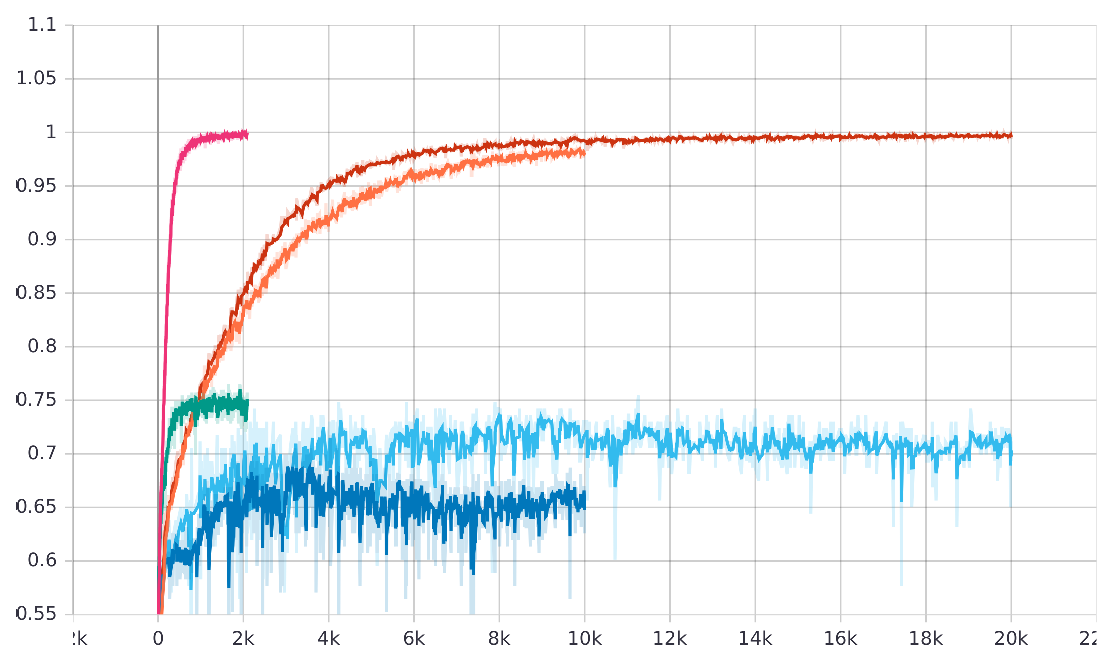
\includegraphics[width=.8\textwidth]{resource/epoch_accuracy.eps}
    \caption{训练-验证准确率}
    \label{Figure.Fourth.2}
  \end{figure}
  \begin{figure}[H]
    \centering
    \includegraphics[width=.8\textwidth]{resource/epoch_loss.eps}
    \caption{训练-验证损失率}
    \label{Figure.Fourth.3}
  \end{figure}

% \subsection{\hei\xiaosan\textbf{模型对比}}
\subsection{\hei\xiaosan\textbf{实验总结}}
  本文提出了一种基于卷积神经网络的小麦病害识别方法。在初步建立该模型后,
  通过优化数据集、改进模型参数以减弱过拟合的影响等方面入手,通过多次实验得到了
  一个表现良好的小麦病害分类模型。
  后期将该模型与经典卷积网络模型LeNet-5、AlexNet等模型进行
  小麦病害识别对比实验,结果表明该模型具有更好的分类识别效果。
  \newpage

  \bibliographystyle{unsrt}
  \bibliography{references}

\end{document}
